\documentclass[12pt]{report}
\usepackage[utf8]{inputenc}
\usepackage[russian]{babel}
\usepackage{setspace} % для междустрочного интервала
\onehalfspacing % 1.5 интервал между строками

\usepackage[left=30mm, top=20mm, right=20mm, bottom=20mm, nohead, footskip=7mm]{geometry}

\usepackage{titlesec, blindtext, color} 
\definecolor{gray75}{gray}{0.75}
\newcommand{\hsp}{\hspace{20pt}}
\titleformat{\chapter}[hang]{\Large\bfseries}{\thechapter{. }}{0pt}{\Large\bfseries}
\titlespacing{\chapter}{-5pt}{-30pt}{12pt} % отступ заголовка сверху
\titleformat{\section}[hang]{\large\bfseries}{\thesection{. }}{0pt}{\large\bfseries}

\makeatletter % список литературы
\def\@biblabel#1{#1. }
\makeatother

% Ссылки
\usepackage{hyperref}

% Возможность вставки pdf страниц
\usepackage{pdfpages}

% Листинги
\usepackage{listings}

\lstset{
	language = c++,
	extendedchars=\true,
	basicstyle=\small\sffamily,
	numbers=left,
	numberstyle=\tiny,
	stepnumber=1,
	numbersep=5pt,
	showspaces=false,            % показывать или нет пробелы специальными отступами
	showstringspaces=false,
	showtabs=false,
	frame=single,
	tabsize=2,
	captionpos=t,
	breaklines=true,
	breakatwhitespace=false,
	escapeinside={\#*}{*)},
	keepspaces=true
}

% Чтобы вместо : в подписях было -
\RequirePackage{caption}
\DeclareCaptionLabelSeparator{defffis}{ — }
\captionsetup{justification=centering,labelsep=defffis}

\usepackage{pgfplots}
\usepackage{pgfplotstable}
\pgfplotsset{compat=1.9}


\begin{document}
	\renewcommand\bibname{Список литературы}
	
	\includepdf[pages=1]{title.pdf}
	
	\tableofcontents
	\newpage
	
	\chapter*{Введение}
	\addcontentsline{toc}{chapter}{Введение}
	\textbf{Трудоёмкость алгоритма} - это зависимость стоимости операций от линейного(ых) размера(ов) входа(ов) \cite{labor_int}.\\

Модель вычислений трудоёмкости должна учитывать следующие оценки.
\begin{itemize}
	\item[1)] Стоимость базовых операций. К ним относятся: =, +, -, *, /, ==, !=, <, <=, >, >=, \%, +=, -=, *=, /=, [ ], < <, > >. Каждая из операций имеет стоимость равную 1.
	\item[2)] Оценка цикла. Она складывается из стоимости тела, инкремента и сравнения. 
	\item[3)] Оценка условного оператора if. Положим, что стоимость перехода к одной из веток равной 0. В таком случае, общая стоимость складывается из подсчета условия и рассмотрения худшего и лучшего случаев.
\end{itemize}

Оценка характера трудоёмкости даётся по наиболее быстрорастущему слагаемому.\\

В этой лабораторной работе будет оцениваться трудоёмкость алгоритмов умножения матриц.
	\newpage
	
	\chapter{Аналитическая часть}
	В этом разделе будут поставлены цель и основные задачи лабораторной работы, которые будут решаться по мере её выполнения.

\section{Цель и задачи}
\qquad\textbf{Цель} данной работы: реализовать и сравнить алгоритмы поиска в словаре.\\

Для достижения поставленной цели необходимо решить следующий ряд \textbf{задач}:
\begin{enumerate}
	\item[1)] дать описание используемого словаря;
	\item[2)] описать алгоритмы поиска;
	\item[3)] реализовать все рассмотренные алгоритмы;
	\item[4)] провести замеры процессорного времени работы алгоритмов;
	\item[5)] найти минимальное/максимальное/среднее время и время работы при несуществующем ключе.
\end{enumerate}

\section{Описание словаря}
\qquadДля этой лабораторной работы был составлен словарь сайтов и паролей к ним, где ключ -- это url сайта, а значение -- пароль.

\section{Используемые алгоритмы поиска}
\qquadБудут использованы следующие алгоритмы поиска ключа.

\subsection{Поиск полным перебором}
\qquadЭтот алгоритм один из самых простых в реализации. В нём используется метод полного перебора, последовательно просматриваются все элементы словаря до тех пор, пока не найдётся соответсвие или пока не проанализуются все возможные варианты. \cite{Kormen}

\subsection{Поиск в упорядоченном словаре двоичным поиском}
\qquadДля этого алгоритма необходимо в качестве подготовительного этапа сначала упорядочить данные. Затем на получившемся наборе производится двоичный поиск ключа, использующий дробление массива на половины. \\

На каждом шаге алгоритма массив данных делится пополам, и дальнейшая работа производится с той частью, где потенциально должно находиться искомое значение. \cite{Tardos}

\subsection{Поиск полным перебором с использованием сегментов}
\qquadВ этом алгоритме производится разбиение исходных данных на сегменты, которые объединены общим признаком. Помимо общих черт, в качестве принципа разделения можно взять частоту обращения к каждому элементу, и на основе анализа частот выделить группы.\\

Для того, чтобы осуществить поиск заданного ключа, необходимо сначала найти сегмент, в котором он может потенциально находится, а затем в этом сегменте попытаться его найти. 

\section*{Вывод}
\addcontentsline{toc}{section}{Вывод}
\qquadБыли поставлены цель и задачи текущей лабораторной работы, также дано краткое описание рассматриваемых алгоритмов.
	\newpage
	
	\chapter{Конструкторская часть}
	Рассмотрим работу алгоритмов на словаре, где каждый элемент имеет следующую структуру: $key$ -- ключ, $value$ -- значение. Длина словаря -- $len$.

\section{Поиск полным перебором}
\qquadОсуществляется поэлементный проход по словарю, и на каждом шаге ключ сравнивается с ключём текущего элемента. Если значения совпали, значит, цель достигнула, элемент найден. В таком случае, алгоритм завершает свою работу. Если же до конца словаря совпадение не было найдено, делается вывод о том, что такого ключа нет.\\

\textbf{Схема} алгоритма представлена на Рис.\ref{fig1:image}.
\begin{figure}[h]
	\begin{center}
		{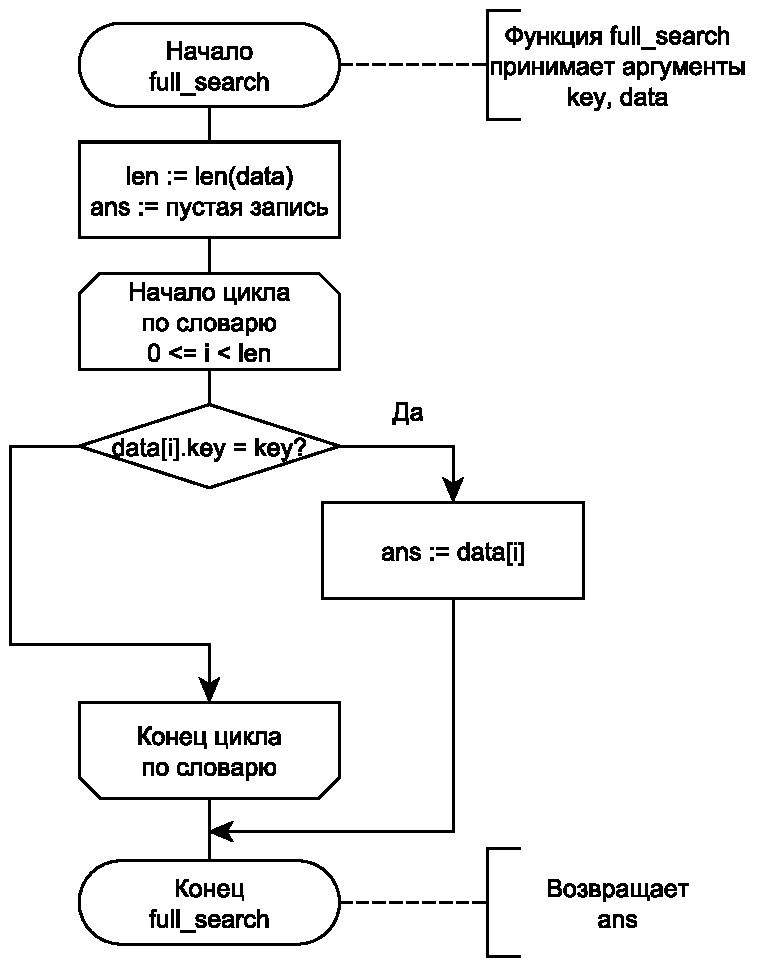
\includegraphics[scale = 0.6]{schemes/full}}
		\caption{Поиск полным перебором}
		\label{fig1:image}
	\end{center}
\end{figure}

\newpage
\section{Поиск в упорядоченном словаре двоичным поиском}
\qquadПеред применением алгоритма нужно предварительно отсортировать массив.
В двоичном поиске вводятся такие понятия как левая ($left$) и правая ($right$) границы массива, индексы которых хранятся в соответствующих переменных. В начале работы алгоритма индекс левой границы равен 0, а правой $len - 1$. На каждой итерации цикла вычисляется индекс элемента, с которым будет производиться сравнение ключа. Находится он по формуле \ref{formula1}.
\begin{equation}\label{formula1}
	middle = \frac{left + right}{2}
\end{equation} 

Если данный ключ больше значения, которое находится по индексу $middle$, то в таком случае левая граница принимает значение $middle + 1$, если меньше, то правая граница становится равной $middle - 1$. В случае совпадения, делается вывод, что нужное значение успешно найдено, и алгоритм завершает свою работу. Если же правая граница становится меньше левой, это свидетельствует о том, что такого ключа в словаре нет, и нужно завершать работу.\\

\textbf{Схема} алгоритма представлена на Рис.\ref{fig2:image}.
\begin{figure}[h]
	\begin{center}
		{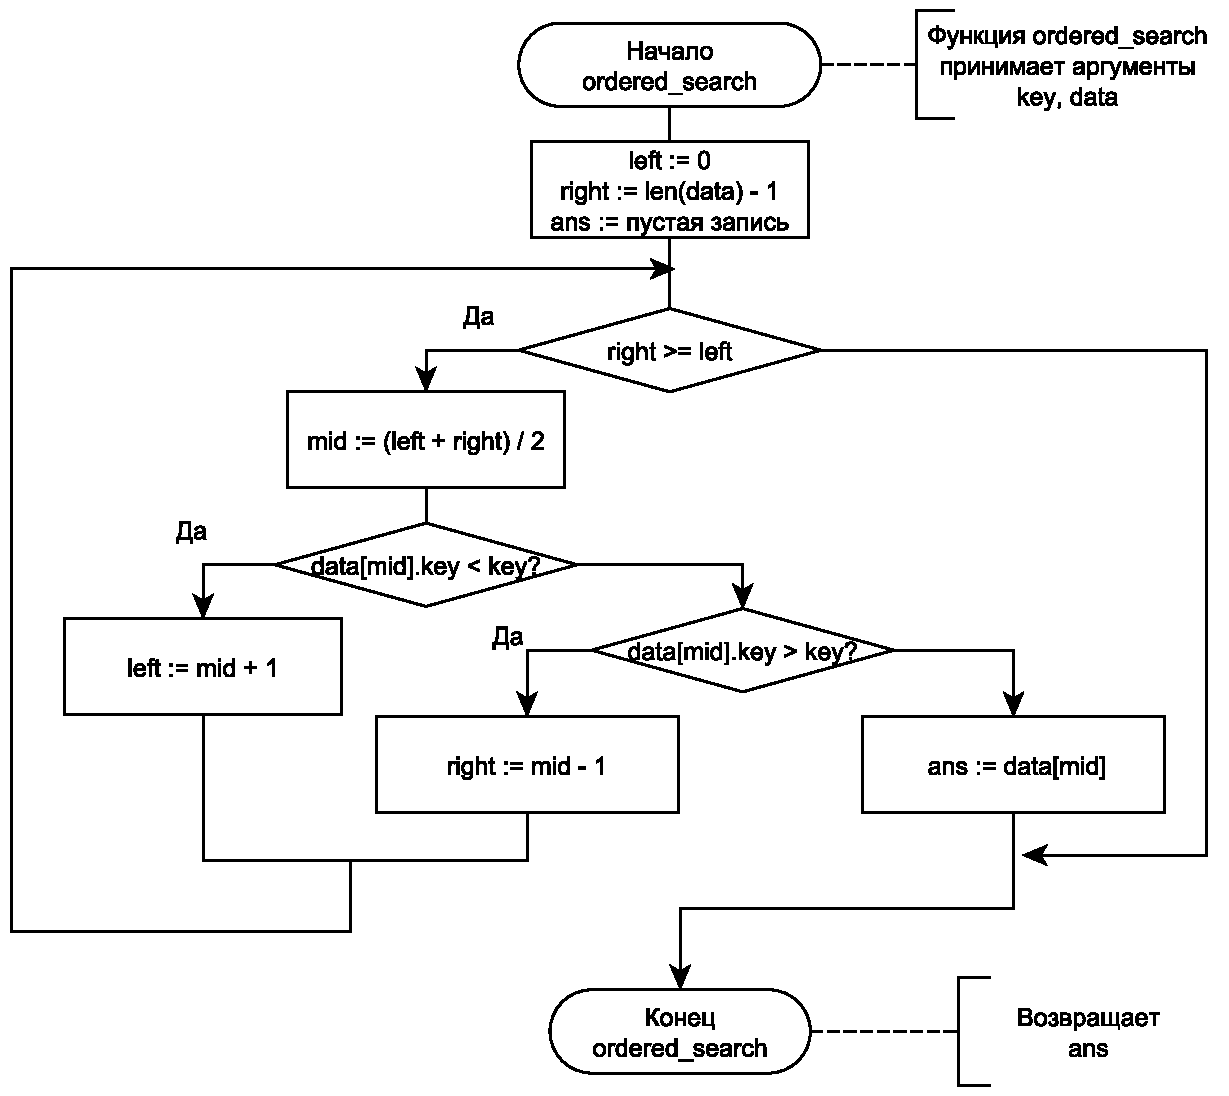
\includegraphics[scale = 0.6]{schemes/sort}}
		\caption{Поиск в упорядоченном словаре двоичным поиском}
		\label{fig2:image}
	\end{center}
\end{figure}

\section{Поиск полным перебором с использованием сегментов}
\qquadДля этого алгоритма также требуется предварительная подготовка -- разбиение словаря на сегменты. В данном случае словарь разбивается по частоте запросов. Будем работать со словарём, в котором url, оканчивающиеся на $ru, com, io$, встречаются примерно одинаковое количество раз,  в то время как $net, biz, org, info$ употреблены в два раза меньше. \\

На основе этого были выделены сегменты с ключами: $\left\{ ru \right\}, \left\{ com \right\}, \left\{ io \right\}, \left\{ net, biz \right\}, \left\{ org, info \right\}$. И на основе этих ключей словарь разделяется на соответствующие сегменты. Каждый из которых состоит из одного из ключей выше и массива элементов словаря (каждый элемент представляет из себя key : value).\\

\textbf{Схема} алгоритма разбиение на сегменты представлена на Рис.\ref{fig3:image}.\\

\newpage

\begin{figure}[pt!]
	\begin{center}
		{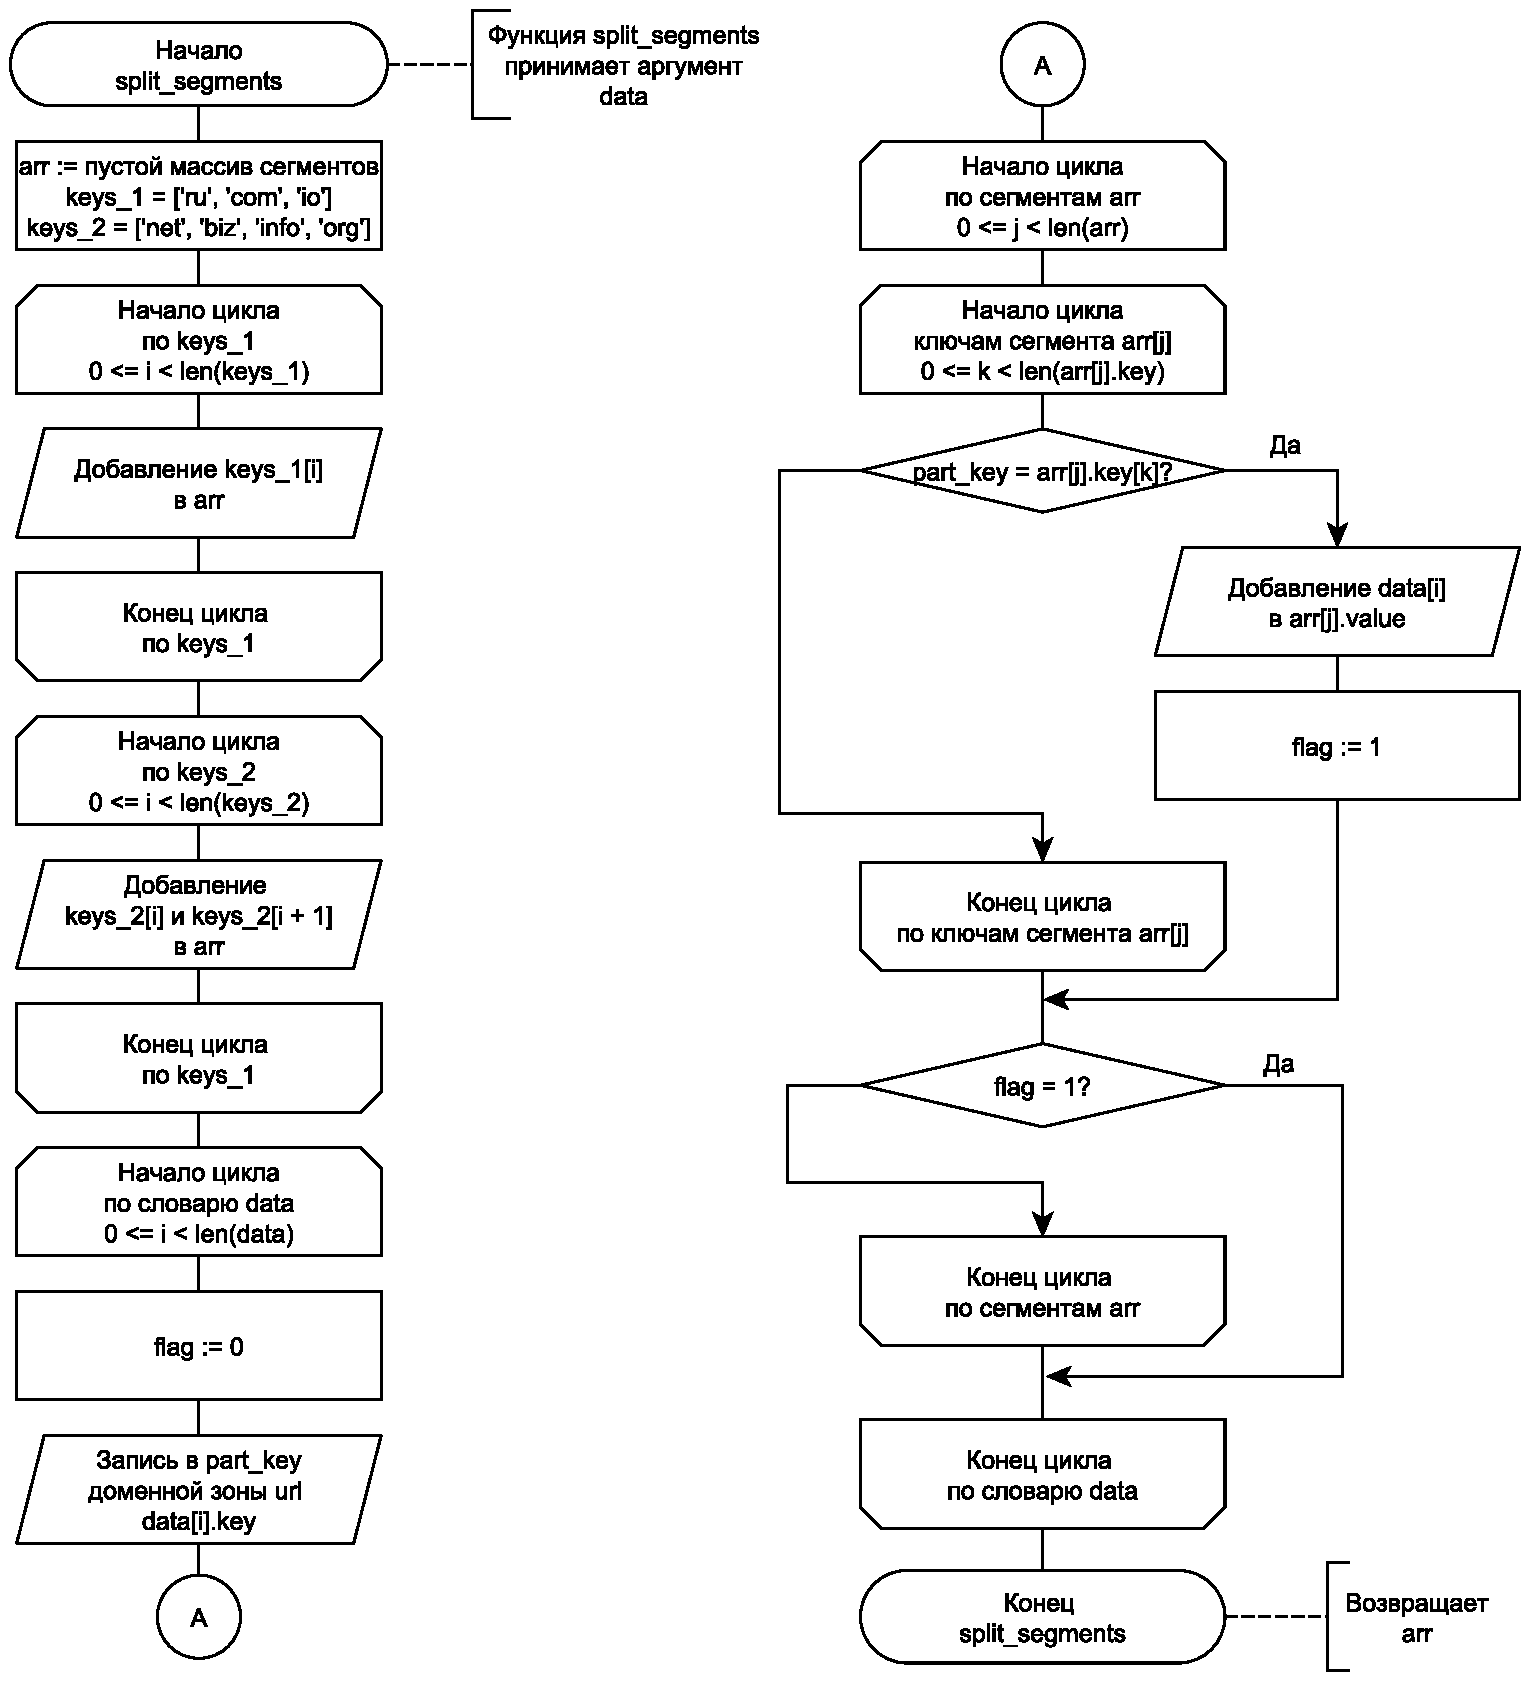
\includegraphics[scale = 0.6]{schemes/split}}
		\caption{Разбиение словаря на сегменты}
		\label{fig3:image}
	\end{center}
\end{figure}

В этом алгоритме сначала находится подходящий сегмент, затем уже внутри сегмента производится последовательный поиск ключа.\\

\textbf{Схема} алгоритма представлена на Рис.\ref{fig4:image}.

\begin{figure}[pt!]
	\begin{center}
		{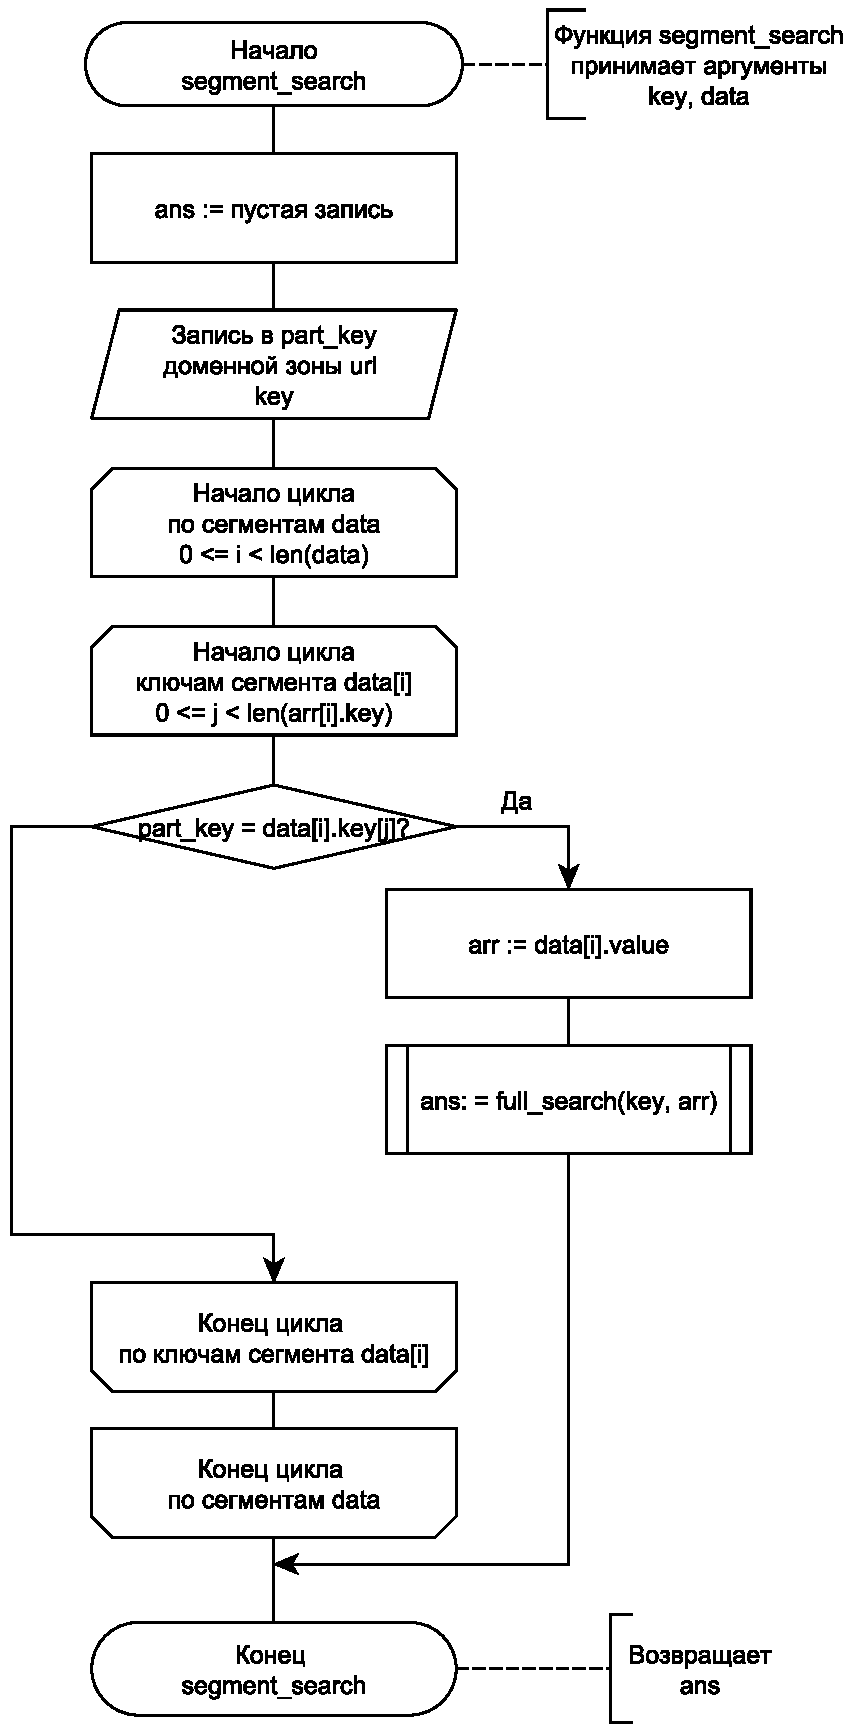
\includegraphics[scale = 0.6]{schemes/segments}}
		\caption{Поиск полным перебором с использованием сегментов}
		\label{fig4:image}
	\end{center}
\end{figure}

\section{Требования к ПО}
\qquadДля корректной работы алгоритмов и проведения тестов необходимо выполнить следующее.
\begin{itemize}
	\item Обеспечить возможность ввода ключа и выбора алгоритма через консоль.
	\item В случае ввода некорректных данных вывести соответствующее сообщение. Программа не должна аварийно завершаться.
	\item Реализовать возможность вывода на экран времени, затрачиваемое на поиск каждого ключа из словаря, а также несуществующего ключа. Вывести максимальное, минимальное и среднее значение.
\end{itemize}

\section{Заготовки тестов}
\qquadПри проверке на корректность работы необходимо провести следующие тесты:
\begin{itemize}
	\item поиск первого элемента словаря;
	\item поиск последнего элемента словаря;
	\item поиск каждого сотого элемента словаря;
	\item поиск несуществующего ключа.
\end{itemize}

\section*{Вывод}
\addcontentsline{toc}{section}{Вывод}
\qquadВ этом разделе разобраны основные принципы выбранных алгоритмов, приведены схемы работы каждого из них, сформулированы требования к программному обеспечению и сделаны заготовки тестов.

	\newpage
	
	\chapter{Технологическая часть}
	В данном разделе будут приведены листинги функций разрабатываемых алгоритмов.

\section{Выбранный язык программирования}
\qquadДля выполнения этой лабораторной работы был выбран язык программирования C++, так как есть большой навык работы с ним и с подключаемыми библиотеками, которые также использовались для проведения тестирования и замеров. \cite{c_plus_plus}

Использованная среда разработки - Visual Studio. \cite{Visual}

\section{Листинг кода}
\qquadНиже представлены Листиги \ref{code1}, \ref{code2} функций, реализующих алгоритмы решения задачи коммивояжёра.

\begin{lstlisting}[label=code1, caption = Алгоритм полного перебора]
matrix_t create_permutations(int n)
{
	vector<int> vct;
	matrix_t res;
	
	for (int i = 0; i < n; i++)
		vct.push_back(i);
	
	res.push_back(vct);
	while (next_permutation(vct.begin(), vct.end()))
		res.push_back(vct);
	
	return res;
}

bool way_is_exist(vector<int> vect, matrix_t& c)
{
	for (int i = 0; i < vect.size(); i++)
		if (c[vect[i]][vect[(i + 1) % vect.size()]] == 0)
			return false;
	
	return true;
}

int find_cost(vector<int> vect, matrix_t& c)
{
	int res = 0;
	
	for (int i = 0; i < vect.size(); i++)
		res += c[vect[i]][vect[(i + 1) % vect.size()]];
	return res;
}

void full_search(matrix_t& c, int n)
{
	vector<int> temp, tour;
	matrix_t prm = create_permutations(n);
	int num = prm.size(), min = 1e5, cost;
	
	for (int i = 0; i < num; i++)
	{
		temp = prm[i];
		if (way_is_exist(temp, c))
		{
			cost = find_cost(temp, c);
			
			if (cost < min)
			{
				min = cost;
				tour = temp;
			}
		}
	}
	
	cout << "Found tour: ";
	for (int i = 0; i < tour.size(); i++)
		cout << tour[i] << " ";
	cout << endl;
	
	cout << "Its length: " << min << endl;
}
\end{lstlisting}

\begin{lstlisting}[label=code2, caption = Муравьиный алгоритм]
matrix_double_t create_pheromone(int n)
{
	matrix_double_t res;
	vector<double> temp;
	
	for (int i = 0; i < n; i++)
	{
		for (int j = 0; j < n; j++)
		temp.push_back(INIT_PHR);
		res.push_back(temp);
	}
	
	return res;
}

double find_avg_path(matrix_t& c)
{
	int n = c.size();
	double res = 0;
	
	for (int i = 0; i < n; i++)
		for (int j = 0; j < n; j++)
			res += c[i][j];
	
	return res / n;
}

vector<ant_t> create_colony(int n)
{
	vector<ant_t> res;
	
	for (int i = 0; i < n; i++)
	{
		ant_t ant;
		ant.done_path.push_back(i);
		ant.cur_pos = i;
		ant.len_path = 0;
		
		res.push_back(ant);
	}
	
	return res;
}

bool is_exist(int index, vector<int> path)
{
	for (int i = 0; i < path.size(); i++)
		if (path[i] == index)
			return true;
	return false;
}

void update_ant(int new_pos, int len, ant_t& ant)
{
	ant.done_path.push_back(new_pos);
	ant.len_path += len;
	ant.cur_pos = new_pos;
}

int find_next_top(matrix_t& c, vector<int>& pos_path, ant_t& ant, matrix_double_t& phr, double a, double b)
{
	int k = 0;
	vector<double> p;
	double p_temp, sum = 0, cur_sum = 0, comp_p;
	
	for (int i = 0; i < pos_path.size(); i++)
	{
		int node = pos_path[i];
		if (c[ant.cur_pos][node])
			p_temp = pow(phr[ant.cur_pos][node], a) / pow(c[ant.cur_pos][node], b);
		else
			p_temp = 0;
		
		p.push_back(p_temp);
		sum += p_temp;
	}
	
	if (sum == 0)
		return -1;
	
	comp_p = (double)rand() / RAND_MAX * sum;
	
	while (cur_sum < comp_p)
	{
		cur_sum += p[k];
		k++;
	}
	
	return k-1;
}

void find_path(matrix_t& c, matrix_double_t& phr, ant_t& ant, double a, double b)
{
	vector<int> pos_path;
	int ind, flag = 1;
	
	for (int i = 0; i < c.size(); i++)
		if (i != ant.cur_pos)
			pos_path.push_back(i);
	
	while (pos_path.size() != 0)
	{
		ind = find_next_top(c, pos_path, ant, phr, a, b);
		if (ind == -1)
			break;
		
		update_ant(pos_path[ind], c[ant.cur_pos][pos_path[ind]], ant);
		
		pos_path.erase(pos_path.begin() + ind);
		if (pos_path.size() == 0 && flag)
		{
			pos_path.push_back(ant.done_path[0]);
			flag = 0;
		}
	}
}

void find_vaporization(matrix_double_t& phr, double k)
{
	for (int i = 0; i < phr.size(); i++)
		for (int j = 0; j < phr[i].size(); j++)
			phr[i][j] = (1 - k) * phr[i][j];
}

void increase_phr(matrix_double_t& pheromone, vector<ant_t> colony, double q)
{
	for (int i = 0; i < colony.size(); i++)
		for (int j = 0; j < colony[i].done_path.size() - 1; j++)
		{
			int node1 = colony[i].done_path[j];
			int node2 = colony[i].done_path[j+1];
			pheromone[node1][node2] += q / colony[i].len_path;
			if (pheromone[node1][node2] < MIN_K_PHR * INIT_PHR)
				pheromone[node1][node2] = MIN_K_PHR * INIT_PHR;
			pheromone[node2][node1] = pheromone[node1][node2];
		}
}

void elite_increase(double q, vector<int>& tour, int len, matrix_double_t& phr)
{
	int num_el_ant = 2;
	
	for (int i = 0; i < tour.size() - 1; i++)
	{
		int node1 = tour[i];
		int node2 = tour[i + 1];
		
		phr[node1][node2] += num_el_ant * q / len;
		phr[node2][node1] += num_el_ant * q / len;
	}
}

void ant_search(double a, double b, matrix_t& c, double k_vpr)
{
	double q = find_avg_path(c);
	matrix_double_t pheromone = create_pheromone(c.size());
	int t_max = 100, len = 1e7;
	vector<int> tour;
	
	for (int t = 0; t < t_max; t++)
	{
		vector<ant_t> colony = create_colony(c.size());
		
		for (int i = 0; i < colony.size(); i++)
		{
			find_path(c, pheromone, colony[i], a, b);
			if (colony[i].len_path < len && colony[i].done_path.size() == c.size() + 1)
			{
				len = colony[i].len_path;
				tour = colony[i].done_path;
			}
		}
		
		find_vaporization(pheromone, k_vpr);
		
		elite_increase(q, tour, len, pheromone);
		
		increase_phr(pheromone, colony, q);
	}
	
	cout << "Found tour: ";
	for (int i = 0; i < tour.size(); i++)
		cout << tour[i] << " ";
	cout << "\nIts length: " << len << endl;
}
\end{lstlisting}

\section{Результаты тестов}
\qquadДля тестирования были написаны функции, проверяющие, согласно заготовкам выше, случаи. Выводы о корректности работы делаются на основе сравнения результатов.\\

\textbf{Все тесты пройдены успешно.} Сами тесты представлены ниже (Листинг \ref{code_test}).\\

\begin{lstlisting}[label=code_test, caption = Тесты]
bool test(matrix_t& c)
{
	vector<int> res1, res2;
	int len1, len2;
	
	len1 = full_search(c, c.size(), res1);
	len2 = ant_search(0.5, 0.5, c, 100, res2);
	
	if (len1 == len2 || res1.size() == 0 && res2.size() == 0)
		return true;
	else
		return false;
}
void test_standart(matrix_t& c)
{
	cout << endl << __FUNCTION__;
	if (test(c))
		cout << ":\tPASSED\n";
	else
		cout << ":\tFAILED\n";
}

void test_size_2(matrix_t& c)
{
	cout << endl << __FUNCTION__;
	if (test(c))
		cout << ":\tPASSED\n";
	else
		cout << ":\tFAILED\n";
}

void test_no_solution(matrix_t& c)
{
	cout << endl << __FUNCTION__;
	if (test(c))
		cout << ":\tPASSED\n";
	else
		cout << ":\tFAILED\n";
}

void test_equal(matrix_t& c)
{
	cout << endl << __FUNCTION__;
	if (test(c))
		cout << ":\tPASSED\n";
	else
		cout << ":\tFAILED\n";
}

void run_tests()
{
	matrix_t c1 = { {0, 1, 2}, {1, 0, 3}, {2, 3, 0} };
	matrix_t c2 = { {0, 10}, {10, 0} };
	matrix_t c3 = { {0, 0, 17}, {0, 0, 0}, {17, 0, 0} };
	matrix_t c4 = { {0, 4, 4}, {4, 0, 4}, {4, 4, 0} };
	
	test_standart(c1);
	test_size_2(c2);
	test_no_solution(c3);
	test_equal(c4);
}	
\end{lstlisting}

\section{Оценка времени}
\qquadПроцессорное время измеряется с помощью функции QueryPerformanceCounter библиотеки windows.h. \cite{Query} Осуществление замеров показано ниже (Листинг \ref{code_time}).

\begin{lstlisting}[label=code_time, caption = Замеры процессорного времени]
	
\end{lstlisting}

\section*{Вывод}
\addcontentsline{toc}{section}{Вывод}
\qquadТаким образом, приведены листинги кода каждой из функций, реализующих алгоритмы решения задачи коммивояжёра, а также листинг тестовых функций, направленных на проверку корректности их работы.

	\newpage
	
	\chapter{Исследовательская часть}
	\section{Характеристики ПО}
\qquadПри проведении замеров времени использовался компьютер, имеющий следующие характеристики:
\begin{itemize}
	\item OC - Windows 10 Pro
	\item Процессор - Inter Core i7 10510U (1800 МГц)
	\item Объём ОЗУ - 16 Гб
\end{itemize}

\section{Измерения}
\qquadДля проведения замеров процессорного времени использовались массивы длин N. \\
$N \in \left\lbrace 10, 50, 100, 500, 1000, 3000, 7000, 10000, 50000, 100000 \right\rbrace$.
Их содержимое генерируется случайным образом.

Каждый замер проводится 5 раз для получения более точного среднего результата.\\

В \hyperref[table_4_1]{таблице 4.1} и \hyperref[table_4_2]{таблице 4.2} представлены результаты замеров процессорного времени работы реализаций алгоритмов (в сек).

\begin{table}[ph] \label{table_4_1}
	\caption{Результаты измерений на размерах до 100 элементов}
	\centering
	\begin{tabular}{|c|c|c|c|}
		\hline
		Размер n&&&\\
		/    &10 &50 & 100 \\
		Алгоритм    &&&\\
		\hline
		Сортировка пузырьком & $1.762\cdot10^{-7}$ & $2.38\cdot10^{-6}$ & $9.066\cdot10^{-6}$ \\
		\hline
		Сортировка вставками & $1.56\cdot10^{-7}$ & $1.687\cdot10^{-6}$ & $6.387\cdot10^{-6}$ \\
		\hline
		Поразрядная сортировка & $1.875\cdot10^{-6}$ & $6.883\cdot10^{-6}$ & $1.328\cdot10^{-5}$ \\
		\hline
	\end{tabular}
\end{table}


\begin{table}[ph] \label{table_4_2}
	\caption{Результаты измерений на размерах до 100 000 элементов}
	\centering
	\begin{tabular}{|c|c|c|c|c|c|c|c|}
		\hline
		Размер n&&&&&&&\\
		/    &500 &1 000 & 3 000 & 7 000 & 10 000 & 50 000 & 100 000 \\
		Алгоритм    &&&&&&&\\
		\hline
		Сортировка & $2.58\cdot10^{-4}$ & $8.53\cdot10^{-4}$ & 0.0077 & 0.043 & 0.089 & 5.924 & 23.705\\
		пузырьком &&&&&&&\\
		\hline
		Сортировка & $1.66\cdot10^{-4}$ & $6.07\cdot10^{-4}$ & 0.0054 & 0.0295 & 0.060 & 1.68 & 7.417\\
		вставками &&&&&&&\\
		\hline
		Поразрядная & $6.452\cdot10^{-5}$ & $1.28\cdot10^{-4}$ & $3.8\cdot10^{-4}$ & $8.9\cdot10^{-4}$ & 0.0013 & 0.0064 & 0.0127\\
		сортировка &&&&&&&\\
		\hline
	\end{tabular}
\end{table}

Согласно полученным результатам можно сделать следующие \textbf{выводы}:
\begin{itemize}
	\item на массивах малого размера (до 100 элементов) поразрядная сортировка показывает результаты по времени примерно на порядок хуже, чем сортировки пузырьком и вставками;
	\item что касается алгоритма сортировки вставками на таких массивах, то среди рассматриваемых трёх алгоритмов у него лучшие показатели по времени;
	\item на массивах большего размера поразрядная сортировка эффективнее, по сравнению с двумя другими алгоритмами, на несколько порядков;
	\item на таких массивах хуже всего показатели по времени у сортировки пузырьком;
	\item сортировка вставками обрабатывает подобные массивы лучше, чем сортировка пузырьком, но значительно уступает по времени поразрядному алгоритму.
\end{itemize}

	\newpage
	
	\chapter*{Заключение}
	\addcontentsline{toc}{chapter}{Заключение}
	В ходе лабораторной работы была достигнута поставленная цель, а именно, проведён сравнительный анализ метода полного перебора и муравьиного алгоритма. \\

В процессе выполнения были решены все задачи. Описаны решаемая задача коммивояжёра, все рассматриваемые алгоритмы. Все проработанные алгоритмы реализованы, кроме того, были проведены замеры процессорного времени работы, оценена трудоёмкость муравьиного алгоритма и проведена его параметризация. На основе полученных данных проведён сравнительный анализ, сделаны выводы.\\

!!!!!!!!!!!!!!!!!!!!!!
	\newpage
	
	\begin{thebibliography}{2}
		\addcontentsline{toc}{chapter}{Список литературы}
		
		\bibitem{Kormen} Кормен, Томас Х. и др Алгоритмы: построение и анализ, 3-е изд. : Пер. с англ. - М. : ООО "И.Д. Вильямс", 2018. - 1328 с. : ил. - Парал. тит. англ. -  ISBN 978-5-8459-2016-4 (рус.).
		
		\bibitem{Tardos} Клейнберг Дж., Тардос Е. Алгоритмы: разработка и применение. Классика Computer Science /Пер. с англ. Е. Матвеева. - СПб.: Питер, 2016. - 800 с.: ил. - (Серия "Классика computer science"). ISBN 978-5-496-01545-5
		
		\bibitem{c_plus_plus} Документация по С++  [Электронный ресурс]. Режим доступа: https://docs.microsoft.com/ru-ru/cpp/cpp/?view=msvc-160, свободный (дата обращения: 22.11.2020)
		
		\bibitem{Visual} Документация по Visual Studio 2019 [Электронный ресурс]. Режим доступа: https://docs.microsoft.com/ru-ru/visualstudio/windows/?view=vs-2019, свободный (дата обращения: 21.11.2020)	
		
		\bibitem{Query} QueryPerformanceCounter function [Электронный ресурс]. Режим доступа: https://docs.microsoft.com/en-us/windows/win32/api/profileapi/nf-profileapi-queryperformancecounter, свободный (дата обращения: 22.11.2020).
	\end{thebibliography}
\end{document}

	\end{thebibliography}
	
\end{document}